% Documents setup
\documentclass[11pt]{book}

% fix for pandoc 1.14
\providecommand{\tightlist}{%
  \setlength{\itemsep}{0pt}\setlength{\parskip}{0pt}}

\usepackage{tabu} % https://tex.stackexchange.com/questions/50332/vertical-spacing-of-a-table-cell

% Location of the csas-style repository: adjust path as needed
\newcommand{\locRepo}{csas-style}

% Use the style file in the csas-style repository (res-doc.sty)
\usepackage{\locRepo/res-doc}

% header-includes from R markdown entry


% Headers and footers
\lhead{}
% \lhead{}
\rhead{}
% \rfoot{DRAFT - DO NOT CITE}

%%%% Commands for title page etc %%%%%

% Publication year
\newcommand{\rdYear}{2021}

% Publication month
\newcommand{\rdMonth}{}

% Report number
\newcommand{\rdNumber}{8}

% Region
\newcommand{\rdRegion}{Pacific Region}

% Title
\newcommand{\rdTitle}{Évaluation des stratégies de rétablissement possibles pour le sébaste aux yeux jaunes (\emph{Sebastes ruberrimus}) des eaux intérieures de la Colombie-Britannique}

\newcommand{\rdISBN}{Fs70-5/2021-008F-PDF}
\newcommand{\rdCatNo}{978-0-660-38699-7}

% Author names separated by commas and ', and' for the last author in the format 'M.H. Grinnell' (use \textsuperscript{n} for addresses)
\newcommand{\rdAuth}{Dana R. Haggarty\textsuperscript{1}, Quang C. Huynh\textsuperscript{2}, Robyn E. Forrest\textsuperscript{1}, Sean C. Anderson\textsuperscript{1}, Midoli J. Bresch\textsuperscript{1}, Elise A. Keppel\textsuperscript{1}}

% Author names reversed separated by commas in the format 'Grinnell, M.H.'
\newcommand{\rdAuthRev}{Haggarty, D.R., C.R. Huynh, R.E. Forrest, S.C. Anderson, M.J. Bresch, et E.A. Keppel}

% Author addresses (use \textsuperscript{n})
\newcommand{\rdAuthAddy}{\textsuperscript{1}Station biologique du Pacifique\\
Pêches et Océans Canada, 3190, chemin Hammond Bay\\
Nanaimo (Colombie-Britannique) V9T 6N7, Canada\\
\textsuperscript{2}Institut pour les océans et la pêche\\
LRAE de l'Université de la Colombie- Britannique, 2202, Main Mall\\
Vancouver (Colombie-Britannique) V6T 1Z4, Canada\\}

\newcommand{\citationOtherLanguage}{Haggarty, D.R., Huynh, Q.C., Forrest, R.E., Anderson, S.C., Bresch, M.J., Keppel, E.A. 2021. Evaluation of potential rebuilding strategies for Inside Yelloweye Rockfish (\emph{Sebastes ruberrimus}) in British Columbia. DFO Can. Sci. Advis. Sec. Res. Doc. 2021/008. vi + 141 p.}

% Name of file with abstract and resume (see \abstract and \frenchabstract for requirements)
\newcommand{\rdAbstract}{\abstract{En vertu des politiques et de la législation canadiennes, il faut Eétablir un plan de rétablissement pour les stocks de poissons qui ont été évalués comme étant inférieurs au point de référence limite (PRL) afin de les ramener au-delà du PRL. Les plans de rétablissement doivent être fondés sur des objectifs caractérisés par 1) une cible, 2) un délai souhaité pour atteindre la cible et 3) une probabilité acceptable d'atteindre la cible. Les plans de rétablissement doivent également comprendre des mesures de gestion ou des procédures de gestion, des jalons cibles et être évalués régulièrement. \vspace{1.5mm} \break Le stock de sébaste aux yeux jaunes (\emph{Sebastes ruberrimus}) des eaux intérieures est un stock sur lequel on dispose de données limitées, présent dans la zone de gestion du poisson de fond 4B (détroit de la Reine-Charlotte, détroit de Georgie et détroit de Juan de Fuca) en Colombie-Britannique. Il a été évalué comme étant inférieur au PLR en 2010, ce qui a donné lieu à la publication d'un plan de rétablissement. Il est également inscrit en vertu de la \emph{Loi sur les espèces en péril} comme espèce préoccupante. L'actuelle procédure de gestion pour assurer le rétablissement est un total autorisé des captures (TAC) annuel fixe de 15 tonnes métriques, qui n'a pas été réévalué depuis la dernière évaluation. \vspace{1.5mm} \break Ce projet vise à fournir un avis scientifique à l'appui de la réévaluation du plan de rétablissement du sébaste aux yeux jaunes des eaux intérieures. Nous appliquons un nouveau cadre d'évaluation de la stratégie de gestion (le Cadre des procédures de gestion), récemment élaboré pour le poisson de fond de la Colombie-Britannique, afin d'évaluer le rendement des autres procédures de gestion à données limitées pour ce qui est de l'atteinte des objectifs de rétablissement. Le Cadre des procédures de gestion suit six étapes de pratiques exemplaires pour évaluer la stratégie de gestion~: 1) la définition du contexte décisionnel; 2) l'établissement des objectifs et des paramètres de rendement; 3) la précision des modèles opérationnels pour représenter le système sous-jacent et calculer les paramètres de rendement; 4) la sélection des procédures de gestion possibles; 5) la réalisation de simulations en boucle fermée afin d'évaluer le rendement des procédures de gestion; 6) la présentation des résultats pour faciliter l'évaluation des compromis. \vspace{1.5mm} \break Nous avons appliqué ce cadre pour évaluer le rendement de 34 procédures de gestion à données limitées pour ce qui est de l'atteinte de l'objectif principal, qui est de ramener le stock au-dessus du PRL sur 1,5 génération avec au moins une probabilité de réussite de 95 \% {[}19 fois sur 20{]}. Nous avons également évalué le rendement des procédures de gestion en ce qui concerne deux autres paramètres de conservation, quatre objectifs de prises moyennes et un objectif de variabilité des prises. Pour tenir compte de l'incertitude liée à la dynamique de la population sous-jacente et aux sources de données, nous avons élaboré six scénarios de modèles opérationnels de rechange, qui différaient de par les hypothèses précises du modèle et des données. Ces scénarios de modèles opérationnels ont été divisés en un « ensemble de référence » (quatre modèles opérationnels) et un « ensemble de robustesse » (deux modèles opérationnels). Nous avons conditionné tous les modèles opérationnels aux données sur les prises observées, aux indices de l'abondance et aux données accessibles sur la composition selon l'âge. Nous avons utilisé la simulation en boucle fermée pour évaluer le rendement des procédures de gestion et nous avons éliminé celles qui ne satisfaisaient pas à un ensemble de critères de base, ce qui a laissé cinq procédures de gestion possibles~: des procédures de gestion à prises constantes annuelles de 10 ou 15 tonnes et trois procédures de gestion qui ajustent le TAC en fonction de la pente relative de l'indice de l'abondance dans le relevé à la palangre sur fond dur dans les eaux intérieures. \vspace{1.5mm} \break Les cinq procédures de gestion finales atteignaient l'objectif principal avec une probabilité supérieure à 0,98 (49 fois sur 50), dans les scénarios des quatre modèles opérationnels de l'ensemble de référence, surtout qu'aucun des modèles opérationnels de l'ensemble de référence n'a estimé que le stock serait inférieur au PRL en 2020. Dans les scénarios des deux modèles opérationnels de l'ensemble de robustesse, le scénario qui simulait une plus grande variabilité dans le futur relevé à la palangre sur fond dur a donné des résultats semblables à ceux des scénarios de l'ensemble de référence. Cependant, dans le scénario qui supposait un taux de mortalité naturelle plus faible pour le stock (« M faible »), toutes les procédures de gestion avaient des probabilités plus basses d'atteindre l'objectif principal, la probabilité la plus faible étant atteinte par la procédure de gestion actuelle (prises constantes de 15 tonnes). \vspace{1.5mm} \break Nous présentons un certain nombre de visualisations pour illustrer les compromis entre les objectifs de conservation et de prises pour les différentes procédures de gestion dans d'autres scénarios de modèles opérationnels. Ces visualisations présentent les compromis sous forme de tableaux et de graphiques, destinés à faciliter le processus de sélection de la procédure de gestion finale. Étant donné que toutes les procédures de gestion ont atteint l'objectif principal dans les scénarios de l'ensemble de référence, il n'y avait pas de compromis important entre les objectifs de conservation et les objectifs de prises. Parmi les deux scénarios de l'ensemble de robustesse, les compromis étaient les plus évidents dans le scénario de M faible, où la probabilité d'atteindre l'objectif principal diminuait à mesure que la probabilité de prises moyennes à court terme de 10 tonnes augmentait. \vspace{1.5mm} \break Nous discutons des incertitudes majeures, y compris l'incertitude entourant la mortalité naturelle, la sélectivité et les prises historiques, en notant que nous avons tenté d'en tenir compte en évaluant le rendement des procédures de gestion dans plusieurs modèles opérationnels. Nous soulignons les problèmes concernant les estimations de l'état actuel du stock de sébaste aux yeux jaunes des eaux intérieures et le rôle des points de référence dans le Cadre des procédures de gestion. Nous formulons des recommandations sur la fréquence des évaluations et suggérons des déclencheurs pour la réévaluation. Nous évaluons également le rendement des procédures de gestion en ce qui concerne le respect de deux autres critères d'évaluation pour le Comité sur la situation des espèces en péril au Canada.}}

%%%% End of title page commands %%%%%

% \pdfcompresslevel=5 % faster PNGs

\setcounter{section}{0}

\bibliographystyle{csas-style/res-doc}

\usepackage{amsmath}
\usepackage{bm}

% commands and environments needed by pandoc snippets
% extracted from the output of `pandoc -s`
%% Make R markdown code chunks work
\usepackage{array}
\usepackage{amssymb,amsmath}
\usepackage{color}
\usepackage{fancyvrb}

% From default template:
\newcommand{\VerbBar}{|}
\newcommand{\VERB}{\Verb[commandchars=\\\{\}]}
\DefineVerbatimEnvironment{Highlighting}{Verbatim}{commandchars=\\\{\}}
% Add ',fontsize=\small' for more characters per line
\usepackage{framed}
\definecolor{shadecolor}{RGB}{248,248,248}
\newenvironment{Shaded}{\begin{snugshade}}{\end{snugshade}}
\newcommand{\AlertTok}[1]{\textcolor[rgb]{0.94,0.16,0.16}{#1}}
\newcommand{\AnnotationTok}[1]{\textcolor[rgb]{0.56,0.35,0.01}{\textbf{\textit{#1}}}}
\newcommand{\AttributeTok}[1]{\textcolor[rgb]{0.77,0.63,0.00}{#1}}
\newcommand{\BaseNTok}[1]{\textcolor[rgb]{0.00,0.00,0.81}{#1}}
\newcommand{\BuiltInTok}[1]{#1}
\newcommand{\CharTok}[1]{\textcolor[rgb]{0.31,0.60,0.02}{#1}}
\newcommand{\CommentTok}[1]{\textcolor[rgb]{0.56,0.35,0.01}{\textit{#1}}}
\newcommand{\CommentVarTok}[1]{\textcolor[rgb]{0.56,0.35,0.01}{\textbf{\textit{#1}}}}
\newcommand{\ConstantTok}[1]{\textcolor[rgb]{0.00,0.00,0.00}{#1}}
\newcommand{\ControlFlowTok}[1]{\textcolor[rgb]{0.13,0.29,0.53}{\textbf{#1}}}
\newcommand{\DataTypeTok}[1]{\textcolor[rgb]{0.13,0.29,0.53}{#1}}
\newcommand{\DecValTok}[1]{\textcolor[rgb]{0.00,0.00,0.81}{#1}}
\newcommand{\DocumentationTok}[1]{\textcolor[rgb]{0.56,0.35,0.01}{\textbf{\textit{#1}}}}
\newcommand{\ErrorTok}[1]{\textcolor[rgb]{0.64,0.00,0.00}{\textbf{#1}}}
\newcommand{\ExtensionTok}[1]{#1}
\newcommand{\FloatTok}[1]{\textcolor[rgb]{0.00,0.00,0.81}{#1}}
\newcommand{\FunctionTok}[1]{\textcolor[rgb]{0.00,0.00,0.00}{#1}}
\newcommand{\ImportTok}[1]{#1}
\newcommand{\InformationTok}[1]{\textcolor[rgb]{0.56,0.35,0.01}{\textbf{\textit{#1}}}}
\newcommand{\KeywordTok}[1]{\textcolor[rgb]{0.13,0.29,0.53}{\textbf{#1}}}
\newcommand{\NormalTok}[1]{#1}
\newcommand{\OperatorTok}[1]{\textcolor[rgb]{0.81,0.36,0.00}{\textbf{#1}}}
\newcommand{\OtherTok}[1]{\textcolor[rgb]{0.56,0.35,0.01}{#1}}
\newcommand{\PreprocessorTok}[1]{\textcolor[rgb]{0.56,0.35,0.01}{\textit{#1}}}
\newcommand{\RegionMarkerTok}[1]{#1}
\newcommand{\SpecialCharTok}[1]{\textcolor[rgb]{0.00,0.00,0.00}{#1}}
\newcommand{\SpecialStringTok}[1]{\textcolor[rgb]{0.31,0.60,0.02}{#1}}
\newcommand{\StringTok}[1]{\textcolor[rgb]{0.31,0.60,0.02}{#1}}
\newcommand{\VariableTok}[1]{\textcolor[rgb]{0.00,0.00,0.00}{#1}}
\newcommand{\VerbatimStringTok}[1]{\textcolor[rgb]{0.31,0.60,0.02}{#1}}
\newcommand{\WarningTok}[1]{\textcolor[rgb]{0.56,0.35,0.01}{\textbf{\textit{#1}}}}

\newcommand{\lt}{\ensuremath <}
\newcommand{\gt}{\ensuremath >}

%Defines cslreferences environment
%Required by pandoc 2.8
%Copied from https://github.com/rstudio/rmarkdown/issues/1649

\DeclareGraphicsExtensions{.png,.pdf}
\begin{document}

\frontmatter

\clearpage

\Appendices


\clearpage

\refstepcounter{chapter}
\label{app:biological-data}
\starredchapter{APPENDIX~\thechapter. DONNÉES BIOLOGIQUES}

Le sébaste aux yeux jaunes des eaux intérieures, qui réside dans la zone 4B (figure~\ref{fig:map-4B}), est génétiquement distinct du stock de sébaste aux yeux jaunes des eaux extérieures, dont l'aire de répartition couvre le reste de la côte (Siegle \protect\hyperlink{ref-siegle2011}{2011}; Siegle et al. \protect\hyperlink{ref-siegle2013}{2013}; Andrews et al. \protect\hyperlink{ref-andrews2018}{2018}). La limite nord entre les deux stocks se trouve au milieu du détroit de la Reine-Charlotte, au nord de l'île Malcolm. La compréhension de la limite sud a changé récemment, d'après les analyses présentées dans Andrews et al. (\protect\hyperlink{ref-andrews2018}{2018}), qui soutiennent que le seuil de Victoria est la limite géologique la plus probable entre les deux populations et que la population des eaux intérieures s'étend dans la baie Puget. On utilise la zone de gestion du poisson de fond 4B pour définir le stock des eaux intérieures, malgré le fait que la zone 4B s'étend au-delà des limites de la population biologique (figure~\ref{fig:map-4B}). Les stocks des eaux intérieures et extérieures sont également considérés comme deux unités désignables distinctes par le COSEPAC (COSEWIC \protect\hyperlink{ref-cosewic2008}{2008}).

\hypertarget{sec:growth}{%
\appsection{ÂGE, TAILLE ET CROISSANCE}\label{sec:growth}}

Le sébaste aux yeux jaunes est une espèce qui vit longtemps et dont l'âge maximal déclaré est de 121 \emph{y} pour le stock des eaux extérieures (Keppel and Olsen \protect\hyperlink{ref-keppel2019}{2019}). L'âge maximal observé pour le stock de sébaste aux yeux jaunes des eaux intérieures est de 101 ans, mis à jour à partir de l'âge maximal de 98 ans signalé précédemment d'après des données récentes supplémentaires sur la détermination de l'âge (figure~\ref{fig:age-freq}). Les données sur l'âge du sébaste aux yeux jaunes des eaux intérieures, dérivées des méthodes de « cassure et brûlage » ou de « cassure et cuisson », sont tirées de divers relevés effectués dans la zone 4B de 1984 à 2018. Les relevés dirigés à la palangre sur fond dur ont commencé dans la zone 4B en 2003, après quoi on a déterminé l'âge de davantage de sébastes aux yeux jaunes. Les proportions selon l'âge du sébaste aux yeux jaunes sont indiquées par année et sexe sur la figure~\ref{fig:age-freq}. On suppose que tous les âges sont indépendants de la sous-zone. Une erreur humaine est possible lors de la lecture de l'âge à partir d'otolithes. La précision de la détermination de l'âge du sébaste aux yeux jaunes des eaux intérieures est indiquée sur la figure~\ref{fig:age-precision}, qui illustre l'âge des poissons déterminé deux fois par des techniciens indépendants, y compris la fourchette d'âges possibles déclarée par chaque technicien.

La longueur maximale du sébaste aux yeux jaunes des eaux intérieures est de 75,9 cm (mâles) et de 76,9 cm (femelles) {[}figure~\ref{fig:length-freq}{]}. Le poids maximal enregistré est de 8,0 kg pour les mâles et les femelles. Les ajustements et les graphiques du modèle longueur-poids pour toutes les données de relevé accessibles sur la zone 4B sont présentés sur la figure~\ref{fig:length-weight}. On suppose que toutes les mesures sont indépendantes de la sous-zone. La courbe longueur-poids prend la forme suivante~:
\begin{equation}
\log (W_i) \sim \operatorname{Student-t}(df = 3, \log(a) + b \log(L_i), \sigma),
\end{equation}
où \(W_i\) et \(L_i\) représentent le poids et la longueur du poisson \(i\), respectivement, et \(\sigma\) représente l'échelle de l'erreur d'observation. Nous avons fixé les degrés de liberté de la loi de Student à 3 pour conférer une certaine robustesse par rapport aux valeurs aberrantes (Anderson et al. \protect\hyperlink{ref-anderson2019synopsis}{2019}). Les variables \(a\) et \(b\) représentent les paramètres longueur-poids estimés. La figure~\ref{fig:length-age} illustre les ajustements et les graphiques du modèle de l'âge selon la longueur pour le sébaste aux yeux jaunes des eaux intérieures. La courbe de croissance de l'âge selon la longueur est un modèle de von Bertalanffy exprimé comme suit~:
\begin{equation}
L_i \sim \operatorname{Log-normal}
\left( \log(l_\mathrm{inf} (1 - \exp(-k (A_i - t_0)))) -
\sigma^2 / 2, \sigma \right),
\end{equation}
où \(L_i\) et \(A_i\) représentent la longueur et l'âge du poisson \(i\), \(l_\mathrm{inf}\), \(k\) et \(t_0\) représentent les paramètres de croissance de von Bertalanffy et \(\sigma\) représente le paramètre d'échelle. Le terme \(- \sigma^2 /2\) représente un terme d'ajustement du biais log-normal, de sorte que nous avons modélisé la longueur moyenne plutôt que la médiane. Le modèle a été ajusté dans Template Model Builder, tel que décrit dans Anderson et al. (\protect\hyperlink{ref-anderson2019synopsis}{2019}).

\hypertarget{sec:maturity}{%
\appsection{MATURITÉ}\label{sec:maturity}}

En plus d'être de grande taille et d'avoir une grande longévité, le sébaste aux yeux jaunes arrive à maturité tardivement. Afin d'examiner l'âge à la maturité, nous avons analysé les enregistrements d'échantillons de tous les relevés menés dans la zone 4B pour trouver des spécimens identifiés comme mâles ou femelles avec un code de maturité valide et dont l'âge a été déterminé selon les méthodes de « cassure et brûlage » ou de « cassure et cuisson ».

Les courbes de maturité sont ajustées en tant que régressions logistiques aux spécimens de poissons individuels, qui sont classés comme étant matures ou non matures en fonction de leur longueur ou de leur âge (figure~\ref{fig:percent-maturity})~:
\begin{align}
y_i &\sim \mathrm{Binomial}(\pi_i)\\
\mathrm{logit} \left( \pi_i \right) &= \beta_0 + \beta_1 x_i + \beta_2 F_i
\end{align}
où \(y_i\) représente un 1 si le poisson \(i\) est considéré comme étant mature et un 0 si le poisson \(i\) est considéré comme étant non mature. Les paramètres \(\beta\) représentent les coefficients estimés, \(x_i\) la longueur ou l'âge du poisson \(i\) et \(F_i\) un prédicteur binaire qui a la valeur 1 si le poisson est une femelle et 0 si le poisson est un mâle. La variable \(\pi_i\) représente la probabilité prévue que le poisson \(i\) soit mature. Les modèles sont ajustés à tous les échantillons de relevé accessibles, quelle que soit la période de l'année. La figure~\ref{fig:prop-mature} illustre les proportions prédites par rapport aux proportions observées de la maturité selon l'âge.



La fréquence de maturité par mois est représentée dans le graphique à bulles de la figure~\ref{fig:mat-months} pour tous les poissons de tous les relevés menés dans la zone 4B pour lesquels la maturité a été échantillonnée. Les catégories de maturité sont présentées du stade le plus immature (en haut) au stade le plus mature (en bas); les poissons individuels, une fois matures, suivent un cycle d'un stade de maturité à l'autre.

\hypertarget{sec:generation}{%
\appsection{DURÉE DE GÉNÉRATION}\label{sec:generation}}

Les directives sur le rétablissement indiquent que le délai de rétablissement doit être de 1,5 à 2 fois la durée de génération de l'espèce (DFO \protect\hyperlink{ref-dfo2013}{2013}), la durée de génération étant le nombre moyen d'années entre la naissance d'un individu et la naissance de sa progéniture. Une analyse récente du stock de sébaste aux yeux jaunes des eaux extérieures a estimé la durée de génération à environ 38 ans, qui était l'âge moyen du stock reproducteur non exploité modélisé (Cox et al. \protect\hyperlink{ref-cox2020}{2020}). Nous avons fixé la durée de génération pour le sébaste aux yeux jaunes des eaux intérieures à un niveau égal à celui estimé pour le stock des eaux extérieures afin d'aligner les calendriers de rétablissement entre les deux stocks.

Toutefois, pour les estimations précédentes de la durée de génération tirées des rapports du COSEPAC et des examens préalables aux évaluations du COSEPAC, on a fait les calculs en utilisant l'âge à la maturité et la mortalité naturelle (âge à 50 \% de la maturité + 1/M). En 2008, on a utilisé un taux de mortalité naturelle de 0,02 et un âge à la maturité de 50 \% de 37,5 ans pour les femelles du stock des eaux intérieures, ce qui a donné une durée de génération estimée à 70 ans (COSEWIC \protect\hyperlink{ref-cosewic2008}{2008}), que l'on considère maintenant comme probablement plus élevée qu'en réalité. En 2018, on a révisé ce chiffre à entre 40,5 et 45,0 ans en utilisant une mortalité naturelle de 0,038 et une maturité de 50 \% de 14,2 à 18,7 ans, estimée à l'aide de données tirées des pêches commerciales et de la recherche, respectivement (Keppel and Olsen \protect\hyperlink{ref-keppel2019}{2019}). En appliquant cette formule et l'estimation médiane de la mortalité naturelle utilisée dans notre modèle opérationnel de référence, 0,045, et la maturité de 50 \% pour le stock des eaux intérieures présentée sur la figure~\ref{fig:percent-maturity}, nous obtenons une durée de génération de 36 pour les femelles et de 40 pour les mâles. Il y a, bien sûr, une grande incertitude associée à l'estimation de la durée de génération à l'aide de cette formule étant donné que la mortalité naturelle est habituellement indiquée comme l'axe principal de l'incertitude dans toutes les évaluations des stocks (p.~ex., Gertseva and Cope (\protect\hyperlink{ref-gertseva2017}{2017}), la présente analyse). Les estimations de la maturité, en particulier la classification des individus matures et non matures selon des méthodes macroscopiques, sont également imprécises (Head et al. \protect\hyperlink{ref-head2016}{2016}). Enfin, les estimations de l'âge sont également sujettes à des erreurs (figure~\ref{fig:age-precision} reproduite d'après l'annexe A du rapport de synthèse des données sur le poisson de fond en Colombie-Britannique (Anderson et al. \protect\hyperlink{ref-anderson2019synopsis}{2019})).

\clearpage


\begin{figure}[htb]

{\centering \pdftooltip{\includegraphics[width=6in]{C:/GitHub/yelloweye-inside/mse/figures-french/age-freq}}{Figure \ref{fig:age-freq}} 

}

\caption{Graphique de la fréquence des âges pour le sébaste aux yeux jaunes des eaux intérieures d'après tous les relevés accessibles menés dans la zone 4B~: relevés à la palangre sur fond dur (nord et sud) dans les eaux intérieures (RPFD INT N/S), relevés à la palangre sur fond dur dans les eaux extérieures (une petite partie de la zone 4B a été incluse dans ce relevé en 2014 et en 2016; RPFD EXT S) et relevés « AUTRES », comprenant les relevés à la turlutte de 1985 et de 1986 et un relevé au chalut de fond en 2005. Les femelles sont représentées par des cercles colorés et les mâles sont représentés derrière par des cercles gris clair. Le nombre total de poissons dont l'âge a été déterminé pour un relevé et une année donnés est indiqué en haut des graphiques. Les lignes diagonales sont affichées à des intervalles de cinq ans pour faciliter le suivi des cohortes dans le temps.}\label{fig:age-freq}
\end{figure}

\begin{figure}[htb]

{\centering \pdftooltip{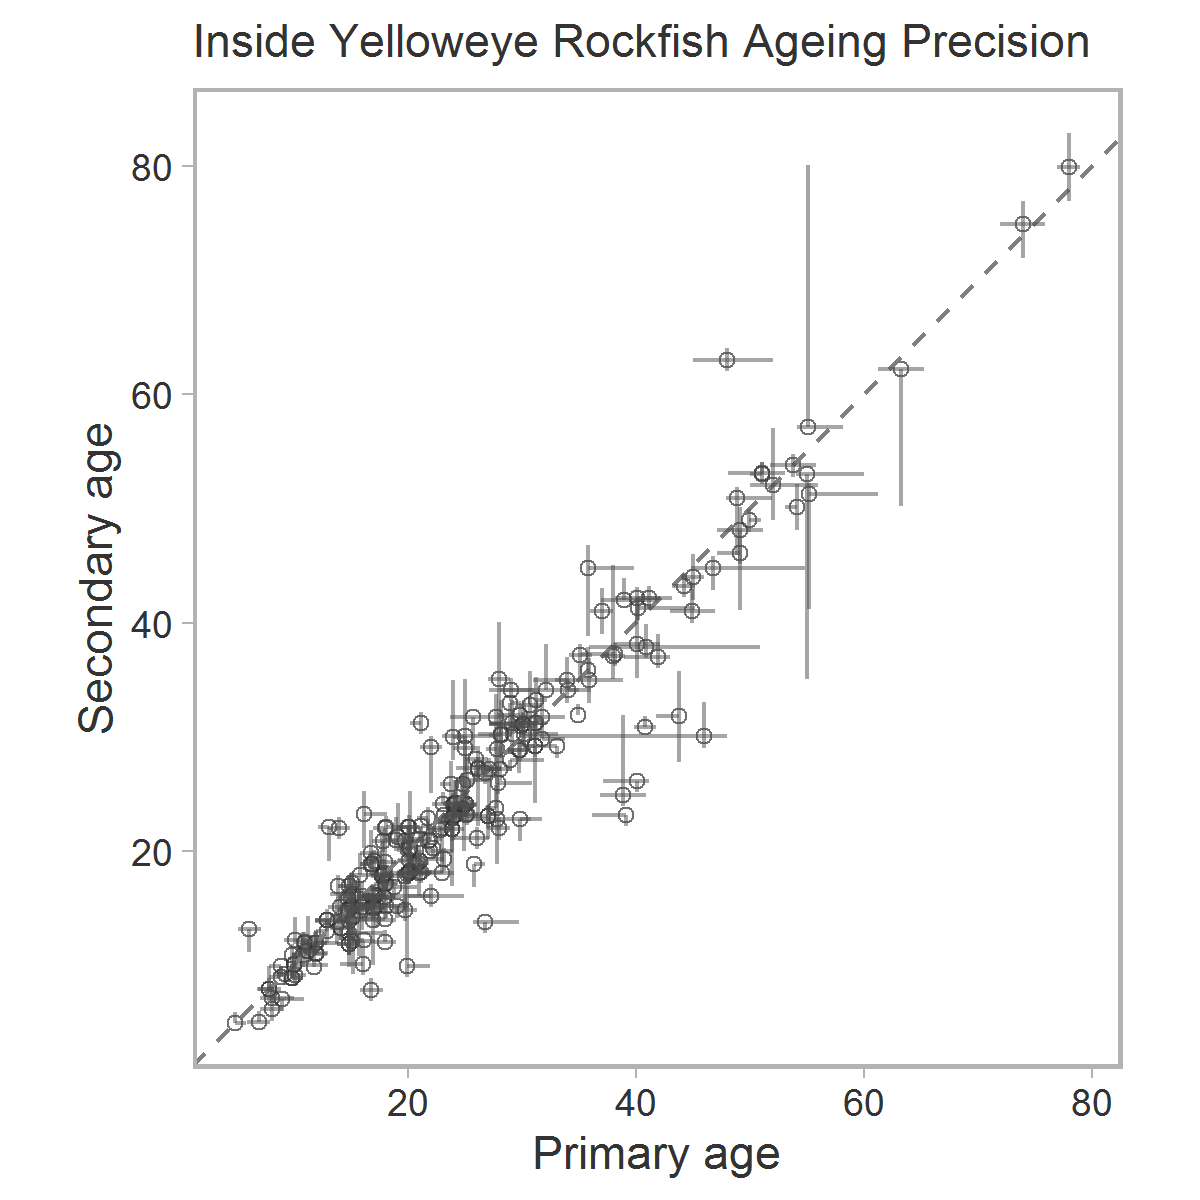
\includegraphics[width=4in]{C:/GitHub/yelloweye-inside/mse/figures-french/ye-ins-age-precision}}{Figure \ref{fig:age-precision}} 

}

\caption{Graphique de précision de la détermination de l'âge pour le sébaste aux yeux jaunes des eaux intérieures. Chaque point et hachure représente un poisson individuel dont l'âge a été déterminé deux fois. L'axe des abscisses représente l'âge et les extrémités supérieures et inférieures de la fourchette des âges possibles enregistrés par le premier lecteur (« principal ») de l'âge des poissons. L'axe des ordonnées représente les valeurs équivalentes enregistrées par le deuxième lecteur (« précision ») de l'âge du poisson. La ligne diagonale tiretée représente un parfait accord un à un entre les deux âges. Parmi tous les sébastes aux yeux jaunes dont l'âge a été déterminé avec précision, 300 poissons ont été échantillonnés au hasard et une petite quantité de fluctuation aléatoire a été ajoutée aux deux axes pour réduire la surreprésentation, la même valeur de fluctuation étant ajoutée aux axes x et y pour un poisson donné.}\label{fig:age-precision}
\end{figure}

\begin{figure}[htb]

{\centering \pdftooltip{\includegraphics[width=5in]{C:/GitHub/yelloweye-inside/mse/figures-french/length-freq}}{Figure \ref{fig:length-freq}} 

}

\caption{Graphiques de la fréquence des longueurs pour le sébaste aux yeux jaunes des eaux intérieures d'après tous les relevés accessibles menés dans la zone 4B~: relevés à la palangre sur fond dur (nord et sud) dans les eaux intérieures (RPFD INT N/S), relevés à la palangre sur fond dur dans les eaux extérieures (une petite partie de la zone 4B a été incluse dans ce relevé en 2014 et en 2016; RPFD EXT S) et relevés « AUTRES », comprenant les relevés à la turlutte de 1985 et de 1986 et un relevé au chalut de fond en 2005. Les poissons femelles sont représentés par des barres colorées et les poissons mâles sont représentés derrière par des barres gris clair. Le nombre total de poissons mesurés pour un relevé et une année donnés est indiqué dans le coin supérieur gauche de chaque graphique.}\label{fig:length-freq}
\end{figure}
\begin{figure}[htb]

{\centering \pdftooltip{\includegraphics[width=0.6\textwidth]{C:/GitHub/yelloweye-inside/mse/figures-french/length-weight}}{Figure \ref{fig:length-weight}} 

}

\caption{Ajustements et graphiques du modèle longueur-poids pour le sébaste aux yeux jaunes des eaux intérieures. Les ajustements du modèle pour les femelles sont indiqués par une ligne pleine noire, et les ajustements du modèle pour les mâles sont indiqués par une ligne grise tiretée. Le texte dans le graphique montre les estimations des paramètres, et les cercles gris ouverts représentent les poissons individuels auxquels les modèles sont ajustés. Tous les échantillons prélevés dans la zone 4B sont compris.}\label{fig:length-weight}
\end{figure}
\begin{figure}[htb]

{\centering \pdftooltip{\includegraphics[width=0.6\textwidth]{C:/GitHub/yelloweye-inside/mse/figures-french/vb}}{Figure \ref{fig:length-age}} 

}

\caption{Ajustements et graphiques du modèle longueur-âge pour le sébaste aux yeux jaunes des eaux intérieures. Les ajustements du modèle sont indiqués pour les femelles par une ligne pleine noire, pour les mâles par une ligne grise tiretée, et pour les sexes combinés par une ligne fine noire. Le texte montre les estimations des paramètres, et les cercles gris ouverts représentent les poissons individuels auxquels les modèles sont ajustés. Tous les échantillons de relevé sont compris.}\label{fig:length-age}
\end{figure}
\begin{figure}[htb]

{\centering \pdftooltip{\includegraphics[width=0.6\textwidth]{C:/GitHub/yelloweye-inside/mse/figures-french/mat-ogive-age}}{Figure \ref{fig:percent-maturity}} 

}

\caption{Courbes de l'âge à la maturité pour le sébaste aux yeux jaunes des eaux intérieures. Les lignes noires pleines représentent les ajustements aux poissons femelles et les lignes grises tiretées, les ajustements aux poissons mâles. Les lignes verticales indiquent l'âge estimé à 50 \% de maturité. Le texte dans les graphiques indique l'âge estimé à 5, 50 et 95 \% de maturité pour les femelles (F) et les mâles (M). Les traits courts en haut et en bas représentent jusqu'à 1 500 poissons choisis au hasard, avec une petite fluctuation aléatoire pour aider à différencier les poissons individuels.}\label{fig:percent-maturity}
\end{figure}

\begin{figure}[htb]

{\centering \pdftooltip{\includegraphics[width=0.6\textwidth]{C:/GitHub/yelloweye-inside/mse/figures-french/mat-prop}}{Figure \ref{fig:prop-mature}} 

}

\caption{Proportions prédites et observées de la maturité selon l'âge chez le sébaste aux yeux jaunes des eaux intérieures.}\label{fig:prop-mature}
\end{figure}

\begin{figure}[htb]

{\centering \pdftooltip{\includegraphics[width=0.6\textwidth]{C:/GitHub/yelloweye-inside/mse/figures-french/mat-months}}{Figure \ref{fig:mat-months}} 

}

\caption{Courbe de la fréquence de maturité par mois pour le sébaste aux yeux jaunes des eaux intérieures. La superficie de chaque cercle correspond au nombre de spécimens de poissons dans une catégorie de maturité donnée pour un mois donné. Les femelles sont indiquées par des cercles noirs et les mâles sont indiqués derrière par des cercles gris clair. Le nombre total de spécimens de poissons pour chaque mois est indiqué par les chiffres figurant en haut du graphique.}\label{fig:mat-months}
\end{figure}
\clearpage

\hypertarget{summary-table-of-biological-data-available}{%
\appsection{SUMMARY TABLE OF BIOLOGICAL DATA AVAILABLE}\label{summary-table-of-biological-data-available}}
\begin{longtable}[]{@{}ccccccc@{}}
\caption{\label{tab:test}Données biologiques sur le sébaste aux yeux jaunes des eaux intérieures.}\tabularnewline
\toprule
Année & Spécimens & Longueurs & Poids & Maturités & Âges & Spécimens d'âge prélevés\tabularnewline
\midrule
\endfirsthead
\toprule
Année & Spécimens & Longueurs & Poids & Maturités & Âges & Spécimens d'âge prélevés\tabularnewline
\midrule
\endhead
1984 & 2 & 1 & 2 & 1 & 0 & 2\tabularnewline
1985 & 87 & 83 & 83 & 86 & 87 & 87\tabularnewline
1986 & 37 & 37 & 37 & 37 & 28 & 37\tabularnewline
1987 & 5 & 5 & 5 & 5 & 0 & 5\tabularnewline
1988 & 12 & 10 & 10 & 12 & 0 & 12\tabularnewline
1992 & 2 & 2 & 2 & 2 & 0 & 2\tabularnewline
1993 & 1 & 1 & 1 & 1 & 0 & 1\tabularnewline
2003 & 135 & 131 & 130 & 107 & 135 & 135\tabularnewline
2004 & 118 & 117 & 115 & 80 & 118 & 118\tabularnewline
2005 & 146 & 141 & 134 & 124 & 146 & 146\tabularnewline
2007 & 65 & 65 & 64 & 53 & 65 & 65\tabularnewline
2008 & 38 & 37 & 30 & 23 & 32 & 38\tabularnewline
2009 & 10 & 10 & 10 & 10 & 8 & 10\tabularnewline
2010 & 153 & 153 & 153 & 145 & 153 & 153\tabularnewline
2011 & 266 & 264 & 264 & 263 & 264 & 266\tabularnewline
2012 & 171 & 170 & 169 & 144 & 169 & 171\tabularnewline
2013 & 223 & 222 & 223 & 209 & 220 & 223\tabularnewline
2014 & 191 & 191 & 190 & 178 & 159 & 191\tabularnewline
2015 & 236 & 232 & 230 & 219 & 209 & 236\tabularnewline
2016 & 257 & 257 & 257 & 247 & 253 & 257\tabularnewline
2018 & 55 & 55 & 55 & 52 & 55 & 55\tabularnewline
\bottomrule
\end{longtable}
\clearpage


\clearpage

\refstepcounter{chapter}
\hypertarget{computational-environment}{%
\starredchapter{APPENDIX~\thechapter. COMPUTATIONAL ENVIRONMENT}\label{computational-environment}}

This version of the document was generated on 2021-10-26 17:03:14 with R version 3.6.3 (2020-02-29) (R Core Team \protect\hyperlink{ref-r2019}{2019}) and R package versions:
\begin{longtable}[]{@{}lll@{}}
\toprule
Package & Version & Date\tabularnewline
\midrule
\endhead
bookdown & 0.17 & 2020-01-11\tabularnewline
cowplot & 1.0.0 & 2019-07-11\tabularnewline
csasdown & 0.0.10.9000 & 2021-05-25\tabularnewline
DLMtool & 5.4.1 & 2019-12-06\tabularnewline
dplyr & 0.8.4 & 2020-01-31\tabularnewline
gfdata & 0.0.0.9000 & 2020-03-04\tabularnewline
gfdlm & 0.0.1.9000 & 2020-03-26\tabularnewline
gfplot & 0.1.4 & 2019-12-10\tabularnewline
ggplot2 & 3.2.1 & 2019-08-10\tabularnewline
knitr & 1.28 & 2020-02-06\tabularnewline
MSEtool & 1.4.3 & 2020-01-10\tabularnewline
purrr & 0.3.3 & 2019-10-18\tabularnewline
rmarkdown & 2.1 & 2020-01-20\tabularnewline
tidyr & 1.0.2 & 2020-01-24\tabularnewline
TMB & 1.7.16 & 2020-01-15\tabularnewline
\bottomrule
\end{longtable}
The source code for this document is available at:\\
\url{https://github.com/pbs-assess/yelloweye-inside/tree/2f9a8a4}.

This document was compiled with the R package csasdown (Anderson et al. \protect\hyperlink{ref-csasdown}{2020}).

The specific versions of the primary packages used to generate this report can be viewed at:

\url{https://github.com/DLMtool/DLMtool/tree/fa971cf}\\
\url{https://github.com/tcarruth/MSEtool/tree/fa1498c}~\\
\url{https://github.com/pbs-assess/gfdata/tree/7292039}~\\
\url{https://github.com/pbs-assess/gfplot/tree/e0b36c0}~\\
\url{https://github.com/pbs-assess/gfdlm/tree/b895686}~\\
\url{https://github.com/pbs-assess/csasdown/tree/f9d5081}~\\

\vspace{4mm}

or installed via:

\texttt{\#\ install.packages(\textquotesingle{}devtools\textquotesingle{})}\\
\texttt{devtools::install\_github(\textquotesingle{}DLMtool/DLMtool\textquotesingle{},\ ref\ =\ \textquotesingle{}fa971cf\textquotesingle{})}~\\
\texttt{devtools::install\_github(\textquotesingle{}tcarruth/MSEtool\textquotesingle{},\ ref\ =\ \textquotesingle{}fa1498c\textquotesingle{})}~\\
\texttt{devtools::install\_github(\textquotesingle{}pbs-assess/gfdata\textquotesingle{},\ ref\ =\ \textquotesingle{}7292039\textquotesingle{})}~\\
\texttt{devtools::install\_github(\textquotesingle{}pbs-assess/sha\_gfplot\textquotesingle{},\ ref\ =\ \textquotesingle{}e0b36c0\textquotesingle{})}~\\
\texttt{devtools::install\_github(\textquotesingle{}pbs-assess/gfdlm\textquotesingle{},\ ref\ =\ \textquotesingle{}b895686\textquotesingle{})}~\\
\texttt{devtools::install\_github(\textquotesingle{}pbs-assess/csasdown\textquotesingle{},\ ref\ =\ \textquotesingle{}f9d5081\textquotesingle{})}~\\

\clearpage

\hypertarget{refs}{}
\leavevmode\hypertarget{ref-csasdown}{}%
Anderson, S.C., Grandin, C., Edwards, A.M., Grinnell, M.H., Ricard, D., and Haigh, R. 2020. csasdown: Reproducible CSAS reports with bookdown. R package version 0.0.8. \url{https://github.com/pbs-assess/csasdown}.

\leavevmode\hypertarget{ref-anderson2019synopsis}{}%
Anderson, S.C., Keppel, E.A., and Edwards, A.M. 2019. A reproducible data synopsis for over 100 species of British Columbia groundfish. DFO Can. Sci. Advis. Sec. Res. Doc. 2019/041 \url{http://www.dfo-mpo.gc.ca/csas-sccs/Publications/ResDocs-DocRech/2019/2019_041-eng.html}.

\leavevmode\hypertarget{ref-andrews2018}{}%
Andrews, K.S., Nichols, K.M., Elz, A., Tolimieri, N., Harvey, C.J., Pacunski, R., Lowry, D., Yamanaka, K.L., and Tonnes, D.M. 2018. Cooperative research sheds light on population structure and listing status of threatened and endangered rockfish species. Conserv. Genet. 19(4): 865--878.

\leavevmode\hypertarget{ref-cosewic2008}{}%
COSEWIC. 2008. COSEWIC assessment and status report on the Yelloweye Rockfish (\emph{Sebastes ruberrimus}), Pacific Ocean inside waters population and Pacific Ocean outside waters population, in Canada. Committee on the Status of Endangered Wildlife in Canada \url{https://www.sararegistry.gc.ca/virtual_sara/files/cosewic/sr_yelloweye_rockfish_0809_e.pdf}.

\leavevmode\hypertarget{ref-cox2020}{}%
Cox, S.P., Doherty, B., Benson, A.J., Johnson, S.D., and Haggarty, D. 2020. Evaluation of potential rebuilding strategies for Outside Yelloweye Rockfish in British Columbia. DFO Can. Sci. Advis. Sec. Res. Doc. 2020/nnn.

\leavevmode\hypertarget{ref-dfo2013}{}%
DFO. 2013. Guidance for the development of rebuilding plans under the Precautionary Approach framework~: Growing stocks out of the critical zone \url{https://www.dfo-mpo.gc.ca/reports-rapports/regs/sff-cpd/precautionary-precaution-eng.htm}.

\leavevmode\hypertarget{ref-gertseva2017}{}%
Gertseva, V., and Cope, J.M. 2017. Stock assessment of the yelloweye rockfish (\emph{Sebastes ruberrimus}) in state and federal waters off California, Oregon and Washington. Pacific Fishery Management Council.

\leavevmode\hypertarget{ref-head2016}{}%
Head, M.A., Stokes, G.L., Thorson, J.T., and Keller, A.A. 2016. Techniques for improving estimates of maturity ogives in groundfish using double-reads and measurement error models. Fish Res. 179: 251--258.

\leavevmode\hypertarget{ref-keppel2019}{}%
Keppel, E.A., and Olsen, N. 2019. Pre-COSEWIC review of Yelloweye Rockfish (\emph{Sebastes ruberrimus}) along the Pacific coast of Canada: Biology, distribution and abundance trends. DFO Can. Sci. Advis. Sec. Res. Doc 2019/014.

\leavevmode\hypertarget{ref-r2019}{}%
R Core Team. 2019. R: A language and environment for statistical computing. R Foundation for Statistical Computing, Vienna, Austria.

\leavevmode\hypertarget{ref-siegle2011}{}%
Siegle, M.R. 2011. Population structure in yelloweye rockfish (\emph{Sebastes ruberrimus}) driven by limited dispersal and selection. Thesis.

\leavevmode\hypertarget{ref-siegle2013}{}%
Siegle, M.R., Taylor, E.B., Miller, K.M., Withler, R.E., and Yamanaka, K.L. 2013. Subtle population genetic structure in Yelloweye Rockfish (\emph{Sebastes ruberrimus}) is consistent with a major oceanographic division in British Columbia, Canada. PLoS ONE 8(8): e71083.

\end{document}
